\chapter{Exploratory Data Analysis}

This chapter presents a comprehensive exploratory analysis of the email dataset generated through the methodological approach described in Chapter 2. The analysis examines multiple dimensions of the corpus to elucidate distinguishing characteristics between spam and legitimate communications.

The initial examination focused on fundamental dataset properties such as dimension and target labels: There are 9353 emails in the dataset with the target labels are 0 for ham and 1 for spam.
The class distribution is 75\% ham and 25\% spam as shown in Figure \ref{Fig:class_distribution}.

\begin{figure}[H]
    \centering
    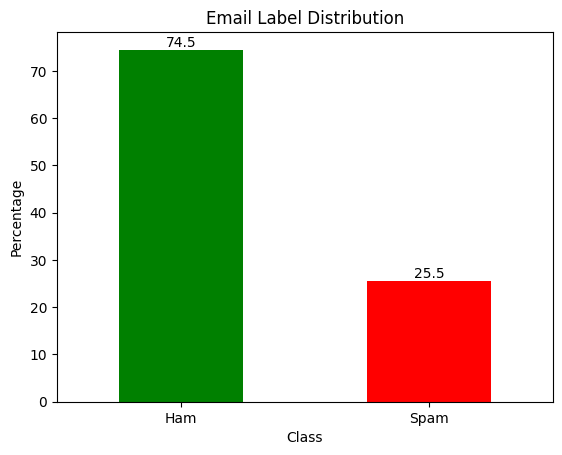
\includegraphics[width=0.7\textwidth]{figures/class_distribution.png}
    \caption{Distribution of ham and spam emails in the dataset}
    \label{Fig:class_distribution}
    \end{figure}

From our preliminary analysis, there are 146 emails out of 9353 which didnt have any value (NaN), it might be due several reasons: blank emails, contain only images with links to some harmful sources, could not be converted from original email or they are not emails, but some other files.
Since the objective of our Case Study is to do the modeling and the number of missing emails are small (~1.5\%), we remove them for now.

A fundamental distinguishing characteristic between spam and legitimate communications is message length.
Bases on the initital dataset, we create a new column called \texttt{word\_count} which is the count of the total number of words the corresponding email content.
We split the collection of emails into two groups: ham and spam.
The analysis revealed distinctive patterns in message length distributions between classes (Figure \ref{fig:length_distribution}): spam messages exhibited higher average length (mean: 352 words); while ham messages showed narrower length variance of 274 words.
Both distributions displayed right skew, with many short messages and fewer very long ones.
These length distribution characteristics suggest message length could serve as a useful feature for classification.

\begin{figure}[H]
\centering
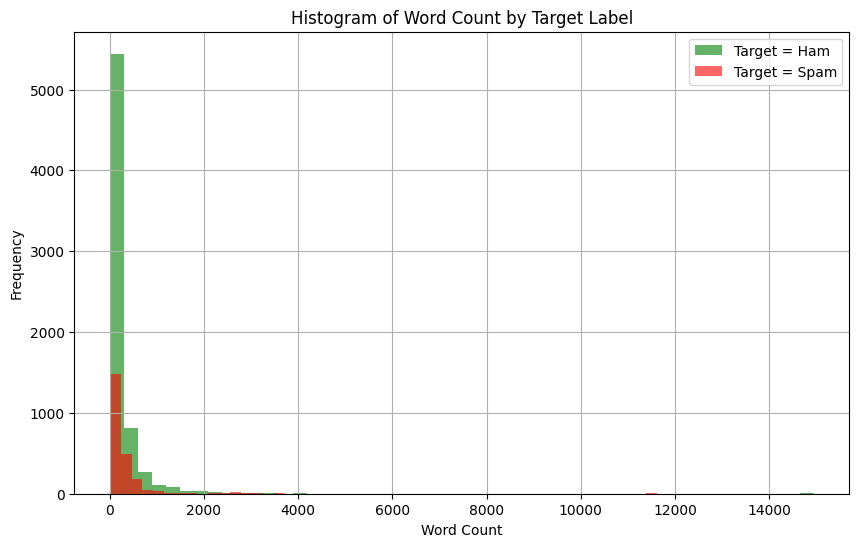
\includegraphics[width=0.9\textwidth]{figures/length_distribution.png}
\caption{Distribution of email lengths by class}
\label{fig:length_distribution}
\end{figure}


In addition to the number of words in the email content, we also count the frequency of each word in the email content.
Finally, we visualize the most common words in each class (Figure \ref{fig:common_words}).

\begin{figure}[H]
\centering
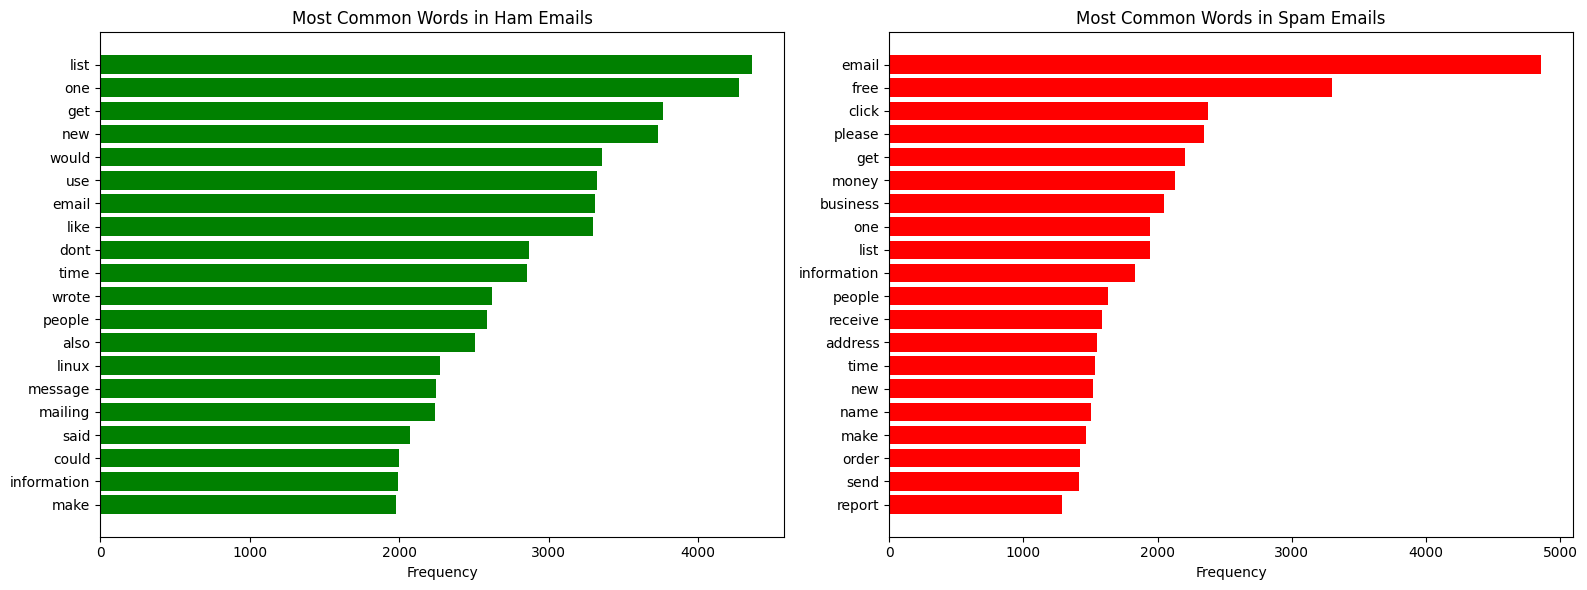
\includegraphics[width=1\textwidth]{figures/common_words.png}
\caption{Most common words in ham and spam emails}
\label{fig:common_words}
\end{figure}

The analysis revealed distinctive lexical characteristics such as ham communications featured more professional and technical vocabulary, spam messages exhibited high frequency of marketing and action-oriented terms and pronoun usage differed significantly between classes

Aggregate lexical patterns were visualized using word clouds to highlight dominant terminology (Figure \ref{fig:wordclouds}):

\begin{figure}[H]
\centering
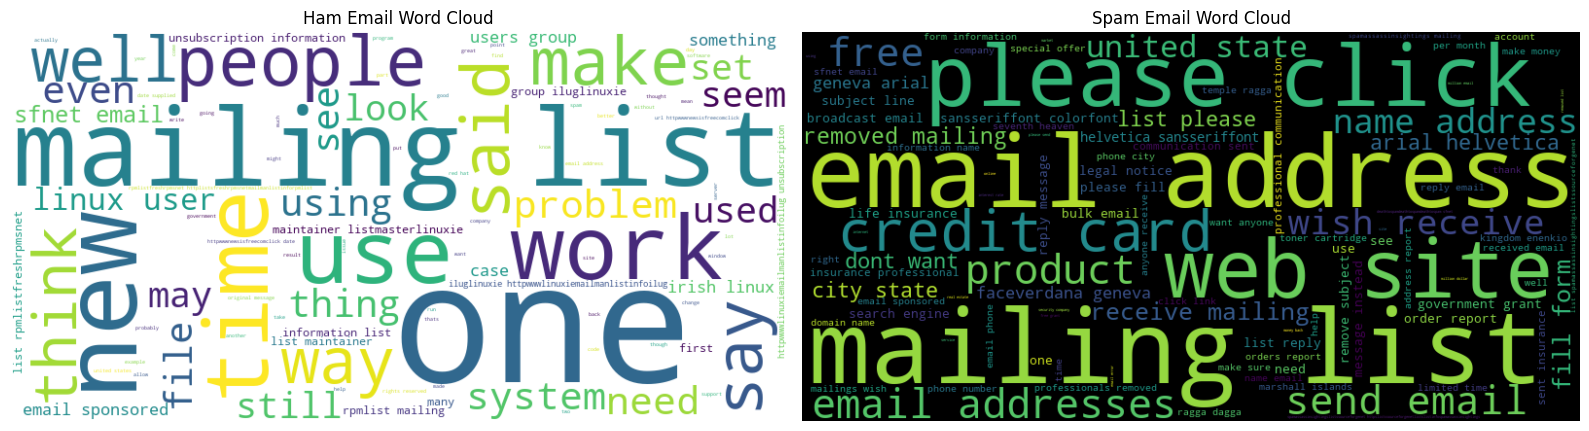
\includegraphics[width=1\textwidth]{figures/wordclouds.png}
\caption{Word clouds for ham (left) and spam (right) emails}
\label{fig:wordclouds}
\end{figure}

The word cloud visualizations reinforced the lexical distinctions observed in frequency analysis while providing additional context regarding semantic domains present in each class.

Communication provenance can provide discriminative signals for classification.
Domain analysis was conducted to identify the most frequent patterns for spam and ham emails (Figure \ref{fig:domain_distribution}):

\begin{figure}[H]
\centering
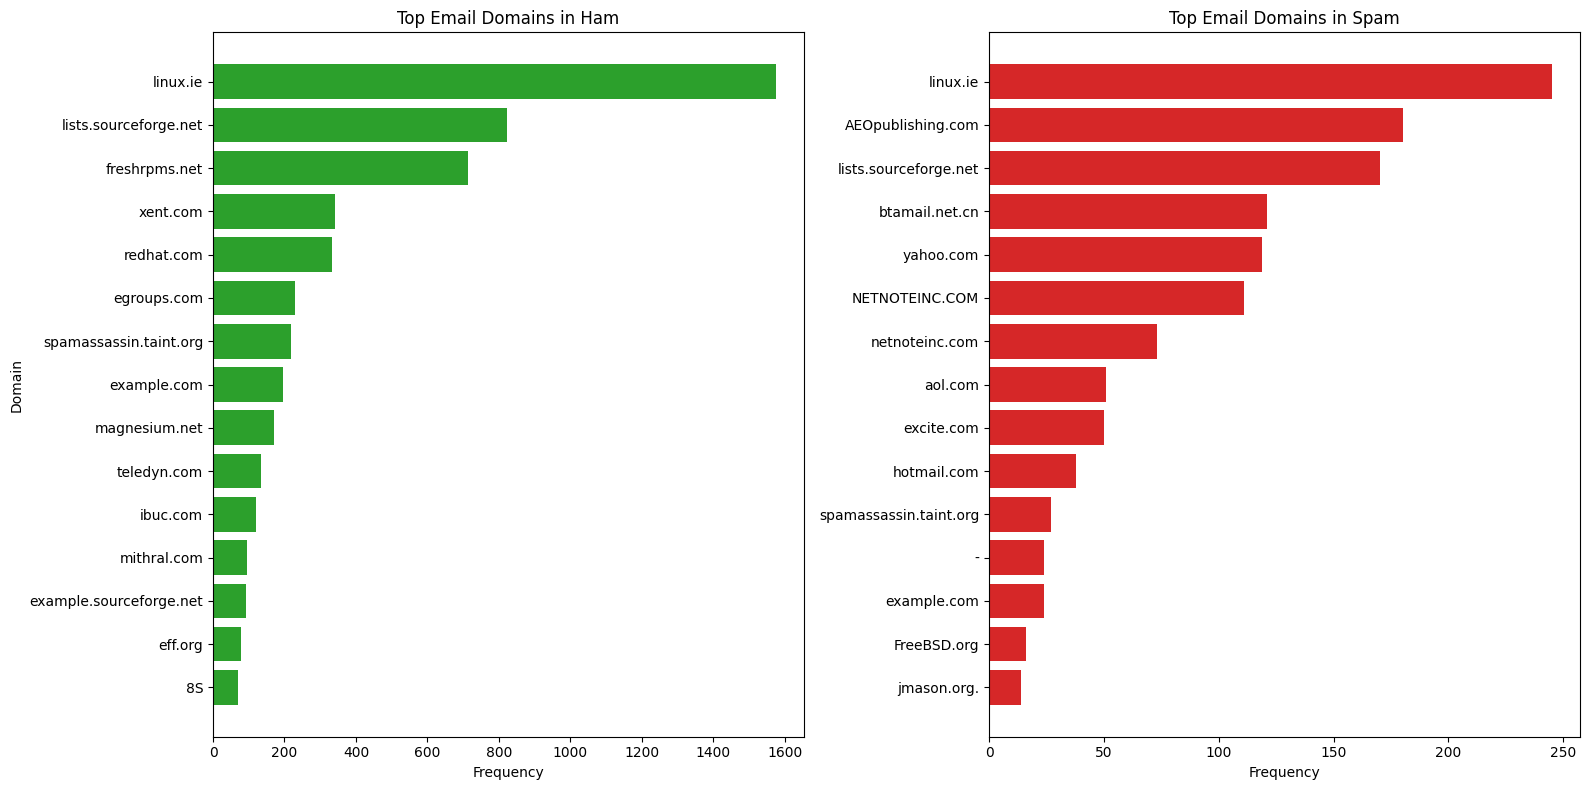
\includegraphics[width=0.9\textwidth]{figures/domain_distribution.png}
\caption{Most common email domains in the dataset}
\label{fig:domain_distribution}
\end{figure}

The domain analysis revealed that high prevalence of free email provider domains in spam communications, correlation between domain reputation and message classification and institutional domains strongly associated with legitimate communications

In conclusion, the exploratory analysis yielded several significant insights:

\begin{enumerate}
    \item Message length characteristics differ substantially between classes
    \item Lexical composition provides strong discriminative signals
    \item Approximately 1.5\% of records contain missing or invalid content
    \item Domain patterns correlate with message classification
\end{enumerate}

These findings inform feature engineering strategies for the subsequent modeling phase, suggesting emphasis on lexical features and appropriate handling of missing values. 